\documentclass[1p]{elsarticle_modified}
%\bibliographystyle{elsarticle-num}

%\usepackage[colorlinks]{hyperref}
%\usepackage{abbrmath_seonhwa} %\Abb, \Ascr, \Acal ,\Abf, \Afrak
\usepackage{amsfonts}
\usepackage{amssymb}
\usepackage{amsmath}
\usepackage{amsthm}
\usepackage{scalefnt}
\usepackage{amsbsy}
\usepackage{kotex}
\usepackage{caption}
\usepackage{subfig}
\usepackage{color}
\usepackage{graphicx}
\usepackage{xcolor} %% white, black, red, green, blue, cyan, magenta, yellow
\usepackage{float}
\usepackage{setspace}
\usepackage{hyperref}

\usepackage{tikz}
\usetikzlibrary{arrows}

\usepackage{multirow}
\usepackage{array} % fixed length table
\usepackage{hhline}

%%%%%%%%%%%%%%%%%%%%%
\makeatletter
\renewcommand*\env@matrix[1][\arraystretch]{%
	\edef\arraystretch{#1}%
	\hskip -\arraycolsep
	\let\@ifnextchar\new@ifnextchar
	\array{*\c@MaxMatrixCols c}}
\makeatother %https://tex.stackexchange.com/questions/14071/how-can-i-increase-the-line-spacing-in-a-matrix
%%%%%%%%%%%%%%%

\usepackage[normalem]{ulem}

\newcommand{\msout}[1]{\ifmmode\text{\sout{\ensuremath{#1}}}\else\sout{#1}\fi}
%SOURCE: \msout is \stkout macro in https://tex.stackexchange.com/questions/20609/strikeout-in-math-mode

\newcommand{\cancel}[1]{
	\ifmmode
	{\color{red}\msout{#1}}
	\else
	{\color{red}\sout{#1}}
	\fi
}

\newcommand{\add}[1]{
	{\color{blue}\uwave{#1}}
}

\newcommand{\replace}[2]{
	\ifmmode
	{\color{red}\msout{#1}}{\color{blue}\uwave{#2}}
	\else
	{\color{red}\sout{#1}}{\color{blue}\uwave{#2}}
	\fi
}

\newcommand{\Sol}{\mathcal{S}} %segment
\newcommand{\D}{D} %diagram
\newcommand{\A}{\mathcal{A}} %arc


%%%%%%%%%%%%%%%%%%%%%%%%%%%%%5 test

\def\sl{\operatorname{\textup{SL}}(2,\Cbb)}
\def\psl{\operatorname{\textup{PSL}}(2,\Cbb)}
\def\quan{\mkern 1mu \triangleright \mkern 1mu}

\theoremstyle{definition}
\newtheorem{thm}{Theorem}[section]
\newtheorem{prop}[thm]{Proposition}
\newtheorem{lem}[thm]{Lemma}
\newtheorem{ques}[thm]{Question}
\newtheorem{cor}[thm]{Corollary}
\newtheorem{defn}[thm]{Definition}
\newtheorem{exam}[thm]{Example}
\newtheorem{rmk}[thm]{Remark}
\newtheorem{alg}[thm]{Algorithm}

\newcommand{\I}{\sqrt{-1}}
\begin{document}

%\begin{frontmatter}
%
%\title{Boundary parabolic representations of knots up to 8 crossings}
%
%%% Group authors per affiliation:
%\author{Yunhi Cho} 
%\address{Department of Mathematics, University of Seoul, Seoul, Korea}
%\ead{yhcho@uos.ac.kr}
%
%
%\author{Seonhwa Kim} %\fnref{s_kim}}
%\address{Center for Geometry and Physics, Institute for Basic Science, Pohang, 37673, Korea}
%\ead{ryeona17@ibs.re.kr}
%
%\author{Hyuk Kim}
%\address{Department of Mathematical Sciences, Seoul National University, Seoul 08826, Korea}
%\ead{hyukkim@snu.ac.kr}
%
%\author{Seokbeom Yoon}
%\address{Department of Mathematical Sciences, Seoul National University, Seoul, 08826,  Korea}
%\ead{sbyoon15@snu.ac.kr}
%
%\begin{abstract}
%We find all boundary parabolic representation of knots up to 8 crossings.
%
%\end{abstract}
%\begin{keyword}
%    \MSC[2010] 57M25 
%\end{keyword}
%
%\end{frontmatter}

%\linenumbers
%\tableofcontents
%
\newcommand\colored[1]{\textcolor{white}{\rule[-0.35ex]{0.8em}{1.4ex}}\kern-0.8em\color{red} #1}%
%\newcommand\colored[1]{\textcolor{white}{ #1}\kern-2.17ex	\textcolor{white}{ #1}\kern-1.81ex	\textcolor{white}{ #1}\kern-2.15ex\color{red}#1	}

{\Large $\underline{12a_{0500}~(K12a_{0500})}$}

\setlength{\tabcolsep}{10pt}
\renewcommand{\arraystretch}{1.6}
\vspace{1cm}\begin{tabular}{m{100pt}>{\centering\arraybackslash}m{274pt}}
\multirow{5}{120pt}{
	\centering
	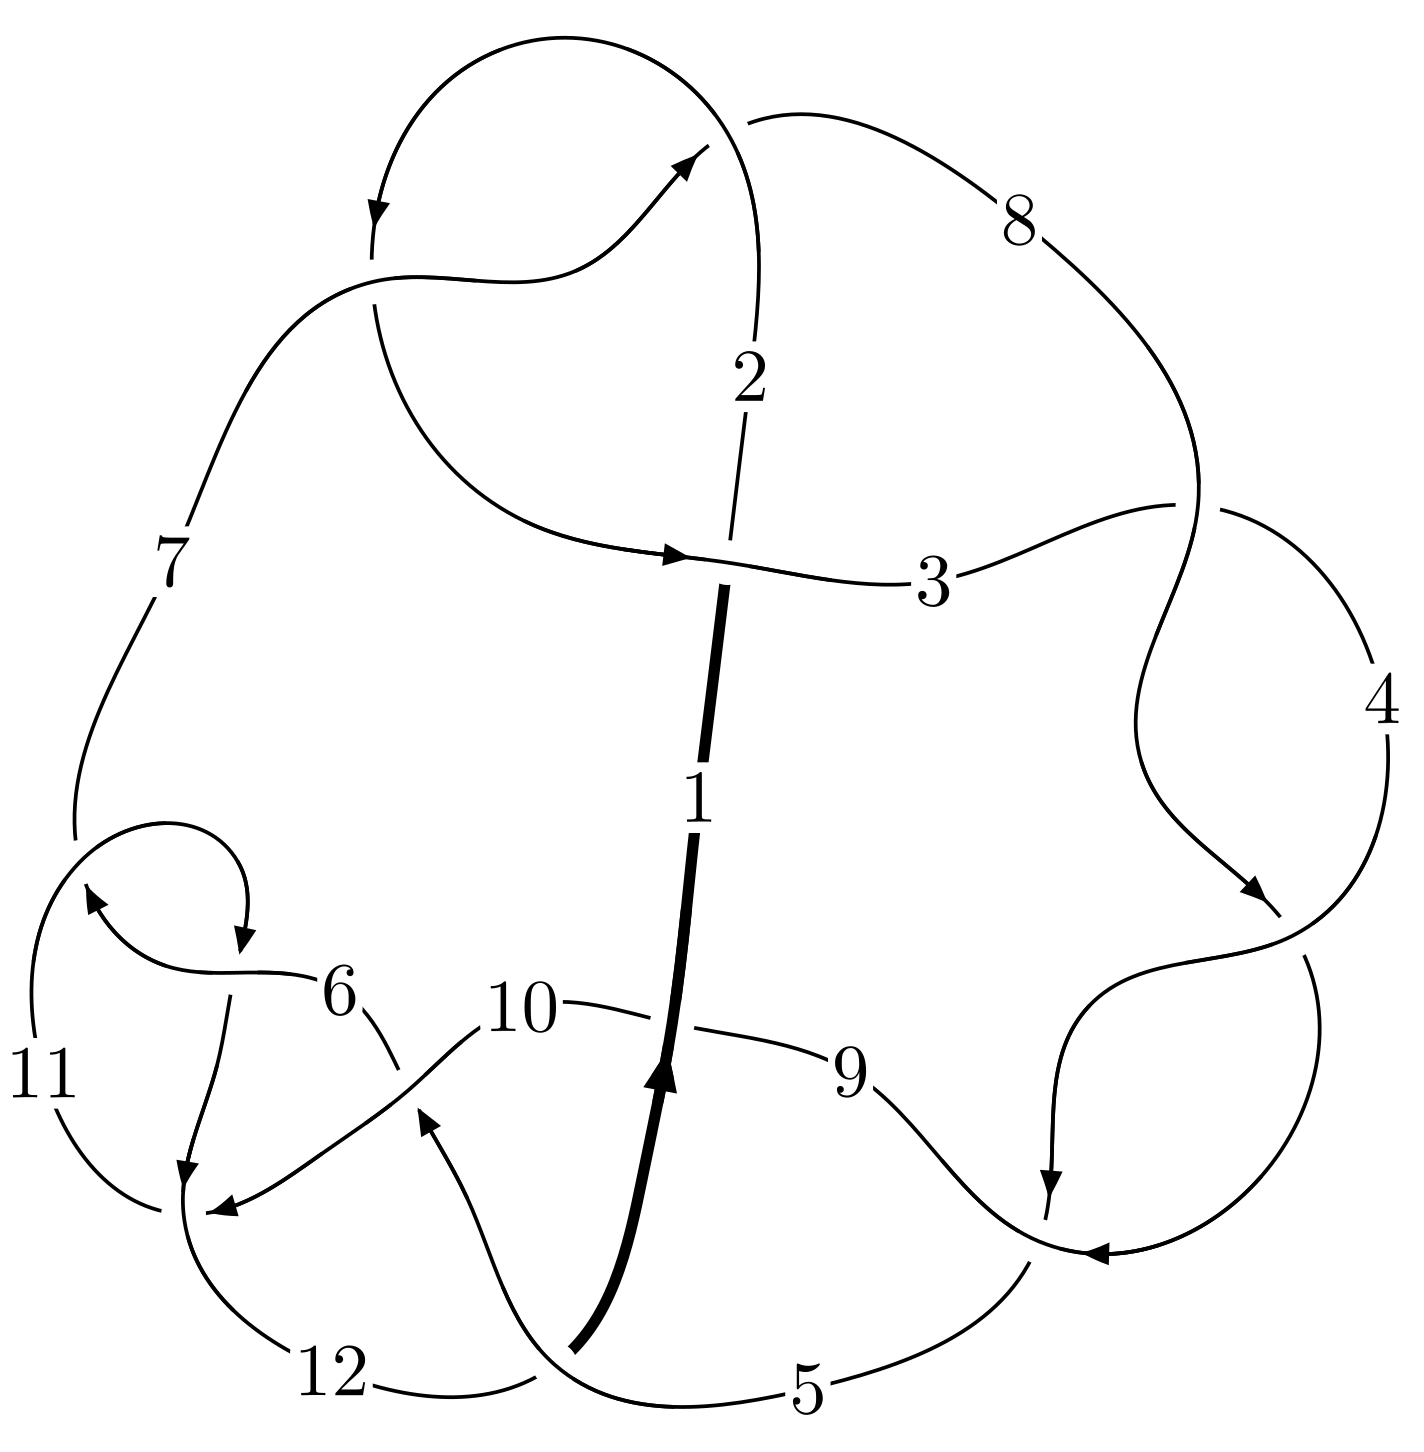
\includegraphics[width=112pt]{../../../GIT/diagram.site/Diagrams/png/1301_12a_0500.png}\\
\ \ \ A knot diagram\footnotemark}&
\allowdisplaybreaks
\textbf{Linearized knot diagam} \\
\cline{2-2}
 &
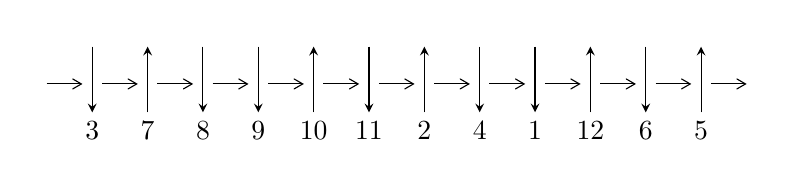
\begin{tikzpicture}[x=20pt, y=17pt]
	% nodes
	\node (C0) at (0, 0) {};
	\node (C1) at (1, 0) {};
	\node (C1U) at (1, +1) {};
	\node (C1D) at (1, -1) {3};

	\node (C2) at (2, 0) {};
	\node (C2U) at (2, +1) {};
	\node (C2D) at (2, -1) {7};

	\node (C3) at (3, 0) {};
	\node (C3U) at (3, +1) {};
	\node (C3D) at (3, -1) {8};

	\node (C4) at (4, 0) {};
	\node (C4U) at (4, +1) {};
	\node (C4D) at (4, -1) {9};

	\node (C5) at (5, 0) {};
	\node (C5U) at (5, +1) {};
	\node (C5D) at (5, -1) {10};

	\node (C6) at (6, 0) {};
	\node (C6U) at (6, +1) {};
	\node (C6D) at (6, -1) {11};

	\node (C7) at (7, 0) {};
	\node (C7U) at (7, +1) {};
	\node (C7D) at (7, -1) {2};

	\node (C8) at (8, 0) {};
	\node (C8U) at (8, +1) {};
	\node (C8D) at (8, -1) {4};

	\node (C9) at (9, 0) {};
	\node (C9U) at (9, +1) {};
	\node (C9D) at (9, -1) {1};

	\node (C10) at (10, 0) {};
	\node (C10U) at (10, +1) {};
	\node (C10D) at (10, -1) {12};

	\node (C11) at (11, 0) {};
	\node (C11U) at (11, +1) {};
	\node (C11D) at (11, -1) {6};

	\node (C12) at (12, 0) {};
	\node (C12U) at (12, +1) {};
	\node (C12D) at (12, -1) {5};
	\node (C13) at (13, 0) {};

	% arrows
	\draw[->,>={angle 60}]
	(C0) edge (C1) (C1) edge (C2) (C2) edge (C3) (C3) edge (C4) (C4) edge (C5) (C5) edge (C6) (C6) edge (C7) (C7) edge (C8) (C8) edge (C9) (C9) edge (C10) (C10) edge (C11) (C11) edge (C12) (C12) edge (C13) ;	\draw[->,>=stealth]
	(C1U) edge (C1D) (C2D) edge (C2U) (C3U) edge (C3D) (C4U) edge (C4D) (C5D) edge (C5U) (C6U) edge (C6D) (C7D) edge (C7U) (C8U) edge (C8D) (C9U) edge (C9D) (C10D) edge (C10U) (C11U) edge (C11D) (C12D) edge (C12U) ;
	\end{tikzpicture} \\
\hhline{~~} \\& 
\textbf{Solving Sequence} \\ \cline{2-2} 
 &
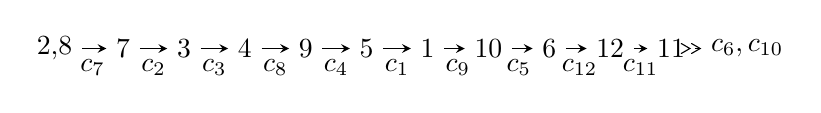
\begin{tikzpicture}[x=22pt, y=7pt]
	% node
	\node (A0) at (-1/8, 0) {2,8};
	\node (A1) at (1, 0) {7};
	\node (A2) at (2, 0) {3};
	\node (A3) at (3, 0) {4};
	\node (A4) at (4, 0) {9};
	\node (A5) at (5, 0) {5};
	\node (A6) at (6, 0) {1};
	\node (A7) at (7, 0) {10};
	\node (A8) at (8, 0) {6};
	\node (A9) at (9, 0) {12};
	\node (A10) at (10, 0) {11};
	\node (C1) at (1/2, -1) {$c_{7}$};
	\node (C2) at (3/2, -1) {$c_{2}$};
	\node (C3) at (5/2, -1) {$c_{3}$};
	\node (C4) at (7/2, -1) {$c_{8}$};
	\node (C5) at (9/2, -1) {$c_{4}$};
	\node (C6) at (11/2, -1) {$c_{1}$};
	\node (C7) at (13/2, -1) {$c_{9}$};
	\node (C8) at (15/2, -1) {$c_{5}$};
	\node (C9) at (17/2, -1) {$c_{12}$};
	\node (C10) at (19/2, -1) {$c_{11}$};
	\node (A11) at (45/4, 0) {$c_{6},c_{10}$};

	% edge
	\draw[->,>=stealth]	
	(A0) edge (A1) (A1) edge (A2) (A2) edge (A3) (A3) edge (A4) (A4) edge (A5) (A5) edge (A6) (A6) edge (A7) (A7) edge (A8) (A8) edge (A9) (A9) edge (A10) ;
	\draw[->>,>={angle 60}]	
	(A10) edge (A11);
\end{tikzpicture} \\ 

\end{tabular} \\

\footnotetext{
The image of knot diagram is generated by the software ``\textbf{Draw programme}" developed by Andrew Bartholomew(\url{http://www.layer8.co.uk/maths/draw/index.htm\#Running-draw}), where we modified some parts for our purpose(\url{https://github.com/CATsTAILs/LinksPainter}).
}\phantom \\ \newline 
\centering \textbf{Ideals for irreducible components\footnotemark of $X_{\text{par}}$} 
 
\begin{align*}
I^u_{1}&=\langle 
u^{83}- u^{82}+\cdots- u^2-1\rangle \\
\\
\end{align*}
\raggedright * 1 irreducible components of $\dim_{\mathbb{C}}=0$, with total 83 representations.\\
\footnotetext{All coefficients of polynomials are rational numbers. But the coefficients are sometimes approximated in decimal forms when there is not enough margin.}
\newpage
\renewcommand{\arraystretch}{1}
\centering \section*{I. $I^u_{1}= \langle u^{83}- u^{82}+\cdots- u^2-1 \rangle$}
\flushleft \textbf{(i) Arc colorings}\\
\begin{tabular}{m{7pt} m{180pt} m{7pt} m{180pt} }
\flushright $a_{2}=$&$\begin{pmatrix}0\\u\end{pmatrix}$ \\
\flushright $a_{8}=$&$\begin{pmatrix}1\\0\end{pmatrix}$ \\
\flushright $a_{7}=$&$\begin{pmatrix}1\\u^2\end{pmatrix}$ \\
\flushright $a_{3}=$&$\begin{pmatrix}u\\u^3+u\end{pmatrix}$ \\
\flushright $a_{4}=$&$\begin{pmatrix}- u^3\\u^3+u\end{pmatrix}$ \\
\flushright $a_{9}=$&$\begin{pmatrix}- u^6- u^4+1\\u^6+2 u^4+u^2\end{pmatrix}$ \\
\flushright $a_{5}=$&$\begin{pmatrix}u^9+2 u^7+u^5-2 u^3- u\\- u^9-3 u^7-3 u^5+u\end{pmatrix}$ \\
\flushright $a_{1}=$&$\begin{pmatrix}u^3\\u^5+u^3+u\end{pmatrix}$ \\
\flushright $a_{10}=$&$\begin{pmatrix}- u^{14}-3 u^{12}-4 u^{10}- u^8+1\\- u^{16}-4 u^{14}-8 u^{12}-8 u^{10}-4 u^8+2 u^6+4 u^4+2 u^2\end{pmatrix}$ \\
\flushright $a_{6}=$&$\begin{pmatrix}- u^{39}-10 u^{37}+\cdots+7 u^7+6 u^5\\- u^{41}-11 u^{39}+\cdots+2 u^3+u\end{pmatrix}$ \\
\flushright $a_{12}=$&$\begin{pmatrix}- u^{23}-6 u^{21}-16 u^{19}-20 u^{17}-4 u^{15}+22 u^{13}+26 u^{11}+6 u^9-9 u^7-6 u^5\\u^{23}+7 u^{21}+\cdots+2 u^3+u\end{pmatrix}$ \\
\flushright $a_{11}=$&$\begin{pmatrix}- u^{62}-17 u^{60}+\cdots+6 u^6+1\\u^{62}+18 u^{60}+\cdots-12 u^6+u^2\end{pmatrix}$\\&\end{tabular}
\flushleft \textbf{(ii) Obstruction class $= -1$}\\~\\
\flushleft \textbf{(iii) Cusp Shapes $= 4 u^{81}-4 u^{80}+\cdots+4 u-2$}\\~\\
\newpage\renewcommand{\arraystretch}{1}
\flushleft \textbf{(iv) u-Polynomials at the component}\newline \\
\begin{tabular}{m{50pt}|m{274pt}}
Crossings & \hspace{64pt}u-Polynomials at each crossing \\
\hline $$\begin{aligned}c_{1}\end{aligned}$$&$\begin{aligned}
&u^{83}+47 u^{82}+\cdots-2 u-1
\end{aligned}$\\
\hline $$\begin{aligned}c_{2},c_{7}\end{aligned}$$&$\begin{aligned}
&u^{83}+u^{82}+\cdots+u^2+1
\end{aligned}$\\
\hline $$\begin{aligned}c_{3},c_{4},c_{8}\end{aligned}$$&$\begin{aligned}
&u^{83}- u^{82}+\cdots+124 u+17
\end{aligned}$\\
\hline $$\begin{aligned}c_{5}\end{aligned}$$&$\begin{aligned}
&u^{83}+u^{82}+\cdots+450 u+317
\end{aligned}$\\
\hline $$\begin{aligned}c_{6},c_{11}\end{aligned}$$&$\begin{aligned}
&u^{83}- u^{82}+\cdots+u^2+1
\end{aligned}$\\
\hline $$\begin{aligned}c_{9}\end{aligned}$$&$\begin{aligned}
&u^{83}-11 u^{82}+\cdots+98 u-29
\end{aligned}$\\
\hline $$\begin{aligned}c_{10}\end{aligned}$$&$\begin{aligned}
&u^{83}-39 u^{82}+\cdots-2 u+1
\end{aligned}$\\
\hline $$\begin{aligned}c_{12}\end{aligned}$$&$\begin{aligned}
&u^{83}-5 u^{82}+\cdots-2422 u+1767
\end{aligned}$\\
\hline
\end{tabular}\\~\\
\newpage\renewcommand{\arraystretch}{1}
\flushleft \textbf{(v) Riley Polynomials at the component}\newline \\
\begin{tabular}{m{50pt}|m{274pt}}
Crossings & \hspace{64pt}Riley Polynomials at each crossing \\
\hline $$\begin{aligned}c_{1}\end{aligned}$$&$\begin{aligned}
&y^{83}-21 y^{82}+\cdots-6 y-1
\end{aligned}$\\
\hline $$\begin{aligned}c_{2},c_{7}\end{aligned}$$&$\begin{aligned}
&y^{83}+47 y^{82}+\cdots-2 y-1
\end{aligned}$\\
\hline $$\begin{aligned}c_{3},c_{4},c_{8}\end{aligned}$$&$\begin{aligned}
&y^{83}-89 y^{82}+\cdots+16906 y-289
\end{aligned}$\\
\hline $$\begin{aligned}c_{5}\end{aligned}$$&$\begin{aligned}
&y^{83}-17 y^{82}+\cdots+3479646 y-100489
\end{aligned}$\\
\hline $$\begin{aligned}c_{6},c_{11}\end{aligned}$$&$\begin{aligned}
&y^{83}+39 y^{82}+\cdots-2 y-1
\end{aligned}$\\
\hline $$\begin{aligned}c_{9}\end{aligned}$$&$\begin{aligned}
&y^{83}-9 y^{82}+\cdots-36274 y-841
\end{aligned}$\\
\hline $$\begin{aligned}c_{10}\end{aligned}$$&$\begin{aligned}
&y^{83}+11 y^{82}+\cdots-14 y-1
\end{aligned}$\\
\hline $$\begin{aligned}c_{12}\end{aligned}$$&$\begin{aligned}
&y^{83}+27 y^{82}+\cdots-121693646 y-3122289
\end{aligned}$\\
\hline
\end{tabular}\\~\\
\newpage\flushleft \textbf{(vi) Complex Volumes and Cusp Shapes}
$$\begin{array}{c|c|c}  
\text{Solutions to }I^u_{1}& \I (\text{vol} + \sqrt{-1}CS) & \text{Cusp shape}\\
 \hline 
\begin{aligned}
u &= -0.133220 + 0.991655 I\end{aligned}
 & \phantom{-}0.112602 - 1.022790 I & \phantom{-0.000000 } 0 \\ \hline\begin{aligned}
u &= -0.133220 - 0.991655 I\end{aligned}
 & \phantom{-}0.112602 + 1.022790 I & \phantom{-0.000000 } 0 \\ \hline\begin{aligned}
u &= \phantom{-}0.464485 + 0.901515 I\end{aligned}
 & \phantom{-}3.37380 + 4.66521 I & \phantom{-0.000000 } 0 \\ \hline\begin{aligned}
u &= \phantom{-}0.464485 - 0.901515 I\end{aligned}
 & \phantom{-}3.37380 - 4.66521 I & \phantom{-0.000000 } 0 \\ \hline\begin{aligned}
u &= \phantom{-}0.460237 + 0.843965 I\end{aligned}
 & \phantom{-}2.23760 - 2.68577 I & \phantom{-}                -6
1.406699 + 0. 10   I\phantom{ +0.000000I} \\ \hline\begin{aligned}
u &= \phantom{-}0.460237 - 0.843965 I\end{aligned}
 & \phantom{-}2.23760 + 2.68577 I & \phantom{-}                -6
1.406699 + 0. 10   I\phantom{ +0.000000I} \\ \hline\begin{aligned}
u &= -0.412629 + 0.867916 I\end{aligned}
 & -0.09451 - 1.65097 I & -2.00000 + 3.87536 I \\ \hline\begin{aligned}
u &= -0.412629 - 0.867916 I\end{aligned}
 & -0.09451 + 1.65097 I & -2.00000 - 3.87536 I \\ \hline\begin{aligned}
u &= \phantom{-}0.180004 + 1.062710 I\end{aligned}
 & -4.06382 - 0.99415 I & \phantom{-0.000000 } 0 \\ \hline\begin{aligned}
u &= \phantom{-}0.180004 - 1.062710 I\end{aligned}
 & -4.06382 + 0.99415 I & \phantom{-0.000000 } 0 \\ \hline\begin{aligned}
u &= -0.158085 + 1.073960 I\end{aligned}
 & -2.03798 + 5.86401 I & \phantom{-0.000000 } 0 \\ \hline\begin{aligned}
u &= -0.158085 - 1.073960 I\end{aligned}
 & -2.03798 - 5.86401 I & \phantom{-0.000000 } 0 \\ \hline\begin{aligned}
u &= -0.481262 + 0.976359 I\end{aligned}
 & \phantom{-}2.43576 - 4.31801 I & \phantom{-0.000000 } 0 \\ \hline\begin{aligned}
u &= -0.481262 - 0.976359 I\end{aligned}
 & \phantom{-}2.43576 + 4.31801 I & \phantom{-0.000000 } 0 \\ \hline\begin{aligned}
u &= \phantom{-}0.240406 + 1.063530 I\end{aligned}
 & -4.57539 + 0.99512 I & \phantom{-0.000000 } 0 \\ \hline\begin{aligned}
u &= \phantom{-}0.240406 - 1.063530 I\end{aligned}
 & -4.57539 - 0.99512 I & \phantom{-0.000000 } 0 \\ \hline\begin{aligned}
u &= -0.272320 + 1.076070 I\end{aligned}
 & -3.03173 - 5.70325 I & \phantom{-0.000000 } 0 \\ \hline\begin{aligned}
u &= -0.272320 - 1.076070 I\end{aligned}
 & -3.03173 + 5.70325 I & \phantom{-0.000000 } 0 \\ \hline\begin{aligned}
u &= \phantom{-}0.442956 + 1.018750 I\end{aligned}
 & -3.12620 + 5.10527 I & \phantom{-0.000000 } 0 \\ \hline\begin{aligned}
u &= \phantom{-}0.442956 - 1.018750 I\end{aligned}
 & -3.12620 - 5.10527 I & \phantom{-0.000000 } 0 \\ \hline\begin{aligned}
u &= \phantom{-}0.481407 + 1.002460 I\end{aligned}
 & -1.91913 + 6.94168 I & \phantom{-0.000000 } 0 \\ \hline\begin{aligned}
u &= \phantom{-}0.481407 - 1.002460 I\end{aligned}
 & -1.91913 - 6.94168 I & \phantom{-0.000000 } 0 \\ \hline\begin{aligned}
u &= -0.405689 + 1.036190 I\end{aligned}
 & -2.06362 - 0.62641 I & \phantom{-0.000000 } 0 \\ \hline\begin{aligned}
u &= -0.405689 - 1.036190 I\end{aligned}
 & -2.06362 + 0.62641 I & \phantom{-0.000000 } 0 \\ \hline\begin{aligned}
u &= -0.493791 + 1.001660 I\end{aligned}
 & \phantom{-}0.34760 - 11.85990 I & \phantom{-0.000000 } 0 \\ \hline\begin{aligned}
u &= -0.493791 - 1.001660 I\end{aligned}
 & \phantom{-}0.34760 + 11.85990 I & \phantom{-0.000000 } 0 \\ \hline\begin{aligned}
u &= \phantom{-}0.869469 + 0.062981 I\end{aligned}
 & -4.54025 - 10.83720 I & -2.95711 + 7.16406 I \\ \hline\begin{aligned}
u &= \phantom{-}0.869469 - 0.062981 I\end{aligned}
 & -4.54025 + 10.83720 I & -2.95711 - 7.16406 I \\ \hline\begin{aligned}
u &= \phantom{-}0.870200 + 0.027576 I\end{aligned}
 & -6.76117 + 1.63137 I & -5.57883 - 2.57822 I \\ \hline\begin{aligned}
u &= \phantom{-}0.870200 - 0.027576 I\end{aligned}
 & -6.76117 - 1.63137 I & -5.57883 + 2.57822 I\\
 \hline 
 \end{array}$$\newpage$$\begin{array}{c|c|c}  
\text{Solutions to }I^u_{1}& \I (\text{vol} + \sqrt{-1}CS) & \text{Cusp shape}\\
 \hline 
\begin{aligned}
u &= -0.869280 + 0.038602 I\end{aligned}
 & -7.89508 + 3.30997 I & -7.43042 - 3.23415 I \\ \hline\begin{aligned}
u &= -0.869280 - 0.038602 I\end{aligned}
 & -7.89508 - 3.30997 I & -7.43042 + 3.23415 I \\ \hline\begin{aligned}
u &= -0.868116 + 0.056802 I\end{aligned}
 & -6.74487 + 5.74130 I & -6.14356 - 3.20858 I \\ \hline\begin{aligned}
u &= -0.868116 - 0.056802 I\end{aligned}
 & -6.74487 - 5.74130 I & -6.14356 + 3.20858 I \\ \hline\begin{aligned}
u &= \phantom{-}0.853560 + 0.057638 I\end{aligned}
 & -2.00681 - 3.24204 I & \phantom{-}0.21808 + 1.91880 I \\ \hline\begin{aligned}
u &= \phantom{-}0.853560 - 0.057638 I\end{aligned}
 & -2.00681 + 3.24204 I & \phantom{-}0.21808 - 1.91880 I \\ \hline\begin{aligned}
u &= \phantom{-}0.809740\phantom{ +0.000000I}\end{aligned}
 & -2.84497\phantom{ +0.000000I} & -3.18540\phantom{ +0.000000I} \\ \hline\begin{aligned}
u &= \phantom{-}0.485858 + 0.628329 I\end{aligned}
 & \phantom{-}2.83112 + 6.65892 I & \phantom{-}2.83091 - 7.70358 I \\ \hline\begin{aligned}
u &= \phantom{-}0.485858 - 0.628329 I\end{aligned}
 & \phantom{-}2.83112 - 6.65892 I & \phantom{-}2.83091 + 7.70358 I \\ \hline\begin{aligned}
u &= -0.274315 + 0.744403 I\end{aligned}
 & -0.270932 - 1.367880 I & -2.47570 + 5.35724 I \\ \hline\begin{aligned}
u &= -0.274315 - 0.744403 I\end{aligned}
 & -0.270932 + 1.367880 I & -2.47570 - 5.35724 I \\ \hline\begin{aligned}
u &= -0.788512 + 0.033384 I\end{aligned}
 & \phantom{-}0.20844 + 3.73783 I & \phantom{-}1.09851 - 4.05017 I \\ \hline\begin{aligned}
u &= -0.788512 - 0.033384 I\end{aligned}
 & \phantom{-}0.20844 - 3.73783 I & \phantom{-}1.09851 + 4.05017 I \\ \hline\begin{aligned}
u &= -0.443590 + 0.624580 I\end{aligned}
 & \phantom{-}0.55457 - 2.06035 I & -0.38344 + 4.13562 I \\ \hline\begin{aligned}
u &= -0.443590 - 0.624580 I\end{aligned}
 & \phantom{-}0.55457 + 2.06035 I & -0.38344 - 4.13562 I \\ \hline\begin{aligned}
u &= \phantom{-}0.480548 + 0.557812 I\end{aligned}
 & \phantom{-}4.32394 - 0.70252 I & \phantom{-}6.01189 - 0.11159 I \\ \hline\begin{aligned}
u &= \phantom{-}0.480548 - 0.557812 I\end{aligned}
 & \phantom{-}4.32394 + 0.70252 I & \phantom{-}6.01189 + 0.11159 I \\ \hline\begin{aligned}
u &= -0.448739 + 1.209870 I\end{aligned}
 & -3.40183 - 0.64725 I & \phantom{-0.000000 } 0 \\ \hline\begin{aligned}
u &= -0.448739 - 1.209870 I\end{aligned}
 & -3.40183 + 0.64725 I & \phantom{-0.000000 } 0 \\ \hline\begin{aligned}
u &= -0.470662 + 1.211330 I\end{aligned}
 & -3.24116 - 8.31020 I & \phantom{-0.000000 } 0 \\ \hline\begin{aligned}
u &= -0.470662 - 1.211330 I\end{aligned}
 & -3.24116 + 8.31020 I & \phantom{-0.000000 } 0 \\ \hline\begin{aligned}
u &= \phantom{-}0.460140 + 1.220060 I\end{aligned}
 & -6.43985 + 4.54605 I & \phantom{-0.000000 } 0 \\ \hline\begin{aligned}
u &= \phantom{-}0.460140 - 1.220060 I\end{aligned}
 & -6.43985 - 4.54605 I & \phantom{-0.000000 } 0 \\ \hline\begin{aligned}
u &= -0.570994 + 0.382917 I\end{aligned}
 & \phantom{-}2.05864 + 7.62104 I & \phantom{-}1.38296 - 6.80721 I \\ \hline\begin{aligned}
u &= -0.570994 - 0.382917 I\end{aligned}
 & \phantom{-}2.05864 - 7.62104 I & \phantom{-}1.38296 + 6.80721 I \\ \hline\begin{aligned}
u &= \phantom{-}0.431215 + 1.244170 I\end{aligned}
 & -5.94329 + 1.26047 I & \phantom{-0.000000 } 0 \\ \hline\begin{aligned}
u &= \phantom{-}0.431215 - 1.244170 I\end{aligned}
 & -5.94329 - 1.26047 I & \phantom{-0.000000 } 0 \\ \hline\begin{aligned}
u &= -0.524837 + 0.426422 I\end{aligned}
 & \phantom{-}3.94874 + 0.21511 I & \phantom{-}5.20374 - 0.31901 I \\ \hline\begin{aligned}
u &= -0.524837 - 0.426422 I\end{aligned}
 & \phantom{-}3.94874 - 0.21511 I & \phantom{-}5.20374 + 0.31901 I \\ \hline\begin{aligned}
u &= \phantom{-}0.489637 + 1.231500 I\end{aligned}
 & -5.52049 + 8.08364 I & \phantom{-0.000000 } 0\\
 \hline 
 \end{array}$$\newpage$$\begin{array}{c|c|c}  
\text{Solutions to }I^u_{1}& \I (\text{vol} + \sqrt{-1}CS) & \text{Cusp shape}\\
 \hline 
\begin{aligned}
u &= \phantom{-}0.489637 - 1.231500 I\end{aligned}
 & -5.52049 - 8.08364 I & \phantom{-0.000000 } 0 \\ \hline\begin{aligned}
u &= \phantom{-}0.428440 + 1.254520 I\end{aligned}
 & -8.55613 - 6.29178 I & \phantom{-0.000000 } 0 \\ \hline\begin{aligned}
u &= \phantom{-}0.428440 - 1.254520 I\end{aligned}
 & -8.55613 + 6.29178 I & \phantom{-0.000000 } 0 \\ \hline\begin{aligned}
u &= -0.432241 + 1.253290 I\end{aligned}
 & -10.73130 + 1.17929 I & \phantom{-0.000000 } 0 \\ \hline\begin{aligned}
u &= -0.432241 - 1.253290 I\end{aligned}
 & -10.73130 - 1.17929 I & \phantom{-0.000000 } 0 \\ \hline\begin{aligned}
u &= -0.443165 + 1.252520 I\end{aligned}
 & -11.81410 - 1.31817 I & \phantom{-0.000000 } 0 \\ \hline\begin{aligned}
u &= -0.443165 - 1.252520 I\end{aligned}
 & -11.81410 + 1.31817 I & \phantom{-0.000000 } 0 \\ \hline\begin{aligned}
u &= \phantom{-}0.449371 + 1.252030 I\end{aligned}
 & -10.64110 + 6.29820 I & \phantom{-0.000000 } 0 \\ \hline\begin{aligned}
u &= \phantom{-}0.449371 - 1.252030 I\end{aligned}
 & -10.64110 - 6.29820 I & \phantom{-0.000000 } 0 \\ \hline\begin{aligned}
u &= -0.492052 + 1.237880 I\end{aligned}
 & -10.2955 - 10.6345 I & \phantom{-0.000000 } 0 \\ \hline\begin{aligned}
u &= -0.492052 - 1.237880 I\end{aligned}
 & -10.2955 + 10.6345 I & \phantom{-0.000000 } 0 \\ \hline\begin{aligned}
u &= \phantom{-}0.495073 + 1.237260 I\end{aligned}
 & -8.0709 + 15.7500 I & \phantom{-0.000000 } 0 \\ \hline\begin{aligned}
u &= \phantom{-}0.495073 - 1.237260 I\end{aligned}
 & -8.0709 - 15.7500 I & \phantom{-0.000000 } 0 \\ \hline\begin{aligned}
u &= -0.483809 + 1.241760 I\end{aligned}
 & -11.51720 - 8.16214 I & \phantom{-0.000000 } 0 \\ \hline\begin{aligned}
u &= -0.483809 - 1.241760 I\end{aligned}
 & -11.51720 + 8.16214 I & \phantom{-0.000000 } 0 \\ \hline\begin{aligned}
u &= \phantom{-}0.478597 + 1.243910 I\end{aligned}
 & -10.42700 + 3.19484 I & \phantom{-0.000000 } 0 \\ \hline\begin{aligned}
u &= \phantom{-}0.478597 - 1.243910 I\end{aligned}
 & -10.42700 - 3.19484 I & \phantom{-0.000000 } 0 \\ \hline\begin{aligned}
u &= \phantom{-}0.546008 + 0.366004 I\end{aligned}
 & -0.17694 - 2.80834 I & -1.96326 + 3.21508 I \\ \hline\begin{aligned}
u &= \phantom{-}0.546008 - 0.366004 I\end{aligned}
 & -0.17694 + 2.80834 I & -1.96326 - 3.21508 I \\ \hline\begin{aligned}
u &= -0.545383 + 0.148864 I\end{aligned}
 & \phantom{-}0.31558 - 3.00332 I & -1.47850 + 2.74614 I \\ \hline\begin{aligned}
u &= -0.545383 - 0.148864 I\end{aligned}
 & \phantom{-}0.31558 + 3.00332 I & -1.47850 - 2.74614 I \\ \hline\begin{aligned}
u &= \phantom{-}0.500212 + 0.257889 I\end{aligned}
 & -1.12463 - 1.27478 I & -4.20587 + 3.81637 I \\ \hline\begin{aligned}
u &= \phantom{-}0.500212 - 0.257889 I\end{aligned}
 & -1.12463 + 1.27478 I & -4.20587 - 3.81637 I\\
 \hline 
 \end{array}$$\newpage
\newpage\renewcommand{\arraystretch}{1}
\centering \section*{ II. u-Polynomials}
\begin{tabular}{m{50pt}|m{274pt}}
Crossings & \hspace{64pt}u-Polynomials at each crossing \\
\hline $$\begin{aligned}c_{1}\end{aligned}$$&$\begin{aligned}
&u^{83}+47 u^{82}+\cdots-2 u-1
\end{aligned}$\\
\hline $$\begin{aligned}c_{2},c_{7}\end{aligned}$$&$\begin{aligned}
&u^{83}+u^{82}+\cdots+u^2+1
\end{aligned}$\\
\hline $$\begin{aligned}c_{3},c_{4},c_{8}\end{aligned}$$&$\begin{aligned}
&u^{83}- u^{82}+\cdots+124 u+17
\end{aligned}$\\
\hline $$\begin{aligned}c_{5}\end{aligned}$$&$\begin{aligned}
&u^{83}+u^{82}+\cdots+450 u+317
\end{aligned}$\\
\hline $$\begin{aligned}c_{6},c_{11}\end{aligned}$$&$\begin{aligned}
&u^{83}- u^{82}+\cdots+u^2+1
\end{aligned}$\\
\hline $$\begin{aligned}c_{9}\end{aligned}$$&$\begin{aligned}
&u^{83}-11 u^{82}+\cdots+98 u-29
\end{aligned}$\\
\hline $$\begin{aligned}c_{10}\end{aligned}$$&$\begin{aligned}
&u^{83}-39 u^{82}+\cdots-2 u+1
\end{aligned}$\\
\hline $$\begin{aligned}c_{12}\end{aligned}$$&$\begin{aligned}
&u^{83}-5 u^{82}+\cdots-2422 u+1767
\end{aligned}$\\
\hline
\end{tabular}\newpage\renewcommand{\arraystretch}{1}
\centering \section*{ III. Riley Polynomials}
\begin{tabular}{m{50pt}|m{274pt}}
Crossings & \hspace{64pt}Riley Polynomials at each crossing \\
\hline $$\begin{aligned}c_{1}\end{aligned}$$&$\begin{aligned}
&y^{83}-21 y^{82}+\cdots-6 y-1
\end{aligned}$\\
\hline $$\begin{aligned}c_{2},c_{7}\end{aligned}$$&$\begin{aligned}
&y^{83}+47 y^{82}+\cdots-2 y-1
\end{aligned}$\\
\hline $$\begin{aligned}c_{3},c_{4},c_{8}\end{aligned}$$&$\begin{aligned}
&y^{83}-89 y^{82}+\cdots+16906 y-289
\end{aligned}$\\
\hline $$\begin{aligned}c_{5}\end{aligned}$$&$\begin{aligned}
&y^{83}-17 y^{82}+\cdots+3479646 y-100489
\end{aligned}$\\
\hline $$\begin{aligned}c_{6},c_{11}\end{aligned}$$&$\begin{aligned}
&y^{83}+39 y^{82}+\cdots-2 y-1
\end{aligned}$\\
\hline $$\begin{aligned}c_{9}\end{aligned}$$&$\begin{aligned}
&y^{83}-9 y^{82}+\cdots-36274 y-841
\end{aligned}$\\
\hline $$\begin{aligned}c_{10}\end{aligned}$$&$\begin{aligned}
&y^{83}+11 y^{82}+\cdots-14 y-1
\end{aligned}$\\
\hline $$\begin{aligned}c_{12}\end{aligned}$$&$\begin{aligned}
&y^{83}+27 y^{82}+\cdots-121693646 y-3122289
\end{aligned}$\\
\hline
\end{tabular}
\vskip 2pc
\end{document}